\documentclass{beamer}
\usepackage{graphicx}
\usepackage{xcolor}
\usepackage{tikz}

% 自定义颜色
\definecolor{purpleblue}{RGB}{80, 80, 180}
\definecolor{lightgray}{RGB}{230, 230, 230}
\definecolor{novelPurple}{RGB}{98, 54, 255} 
\definecolor{darkgray}{RGB}{50, 50, 50}

% 主题设置
\usetheme{Madrid}  
\usecolortheme{dolphin} 

% 设置字体（移除 fontspec，确保 pdfLaTeX 兼容）
\setbeamerfont{title}{size=\Large,series=\bfseries}
\setbeamerfont{frametitle}{size=\LARGE,series=\bfseries}
\setbeamercolor{frametitle}{fg=white, bg=novelPurple}
\setbeamercolor{title}{fg=white, bg=purpleblue}

% 封面信息
\title[SAT Hard Question]{\textbf{SAT Hard Question 3}}
\author{\textbf{Jack Zeng}}
\institute{\textcolor{white}{\textbf{Novel Prep}}}
\date{\today} 

\begin{document}

% --- Title Slide ---
\begin{frame}
    \titlepage
    \vfill
    \begin{flushright}
        \textcolor{purpleblue}{\Huge \textbf{Novel Prep}}
    \end{flushright}
\end{frame}


\begin{frame}
    \begin{tikzpicture}[remember picture, overlay]
        % 设置浅色渐变背景
        \shade[top color=softPurple, bottom color=softGray] 
            (current page.north west) rectangle (current page.south east);
        
        % 添加高斯模糊光晕
        \fill[white, opacity=0.3] (current page.center) circle (4cm);
        
        % 主标题
        \node[align=center] at (current page.center) {
            {\Huge\bfseries\textcolor{purpleblue}{Novel Prep}} \\[0.5cm]
            {\Large\itshape\textcolor{lightText}{Excellence in SAT Prep}}
        };

        % 添加柔和光点（点缀）
        \foreach \x in {1,2,3,4,5} {
            \fill[purpleblue, opacity=0.2] (rand*10-5, rand*7-3.5) circle (0.1+\x*0.05);
        }

        ;
    \end{tikzpicture}
\end{frame}

% Question 14
\begin{frame}{Statistical Sampling and Margin of Error}
\small
A research manager selected 2 random samples of ovens of a certain type to estimate the average amount of time this type of oven takes to preheat to $325^\circ F$. The research manager recorded the amount of time, in minutes, each oven takes to preheat to $325^\circ F$.

Based on the first sample, the manager estimated an average of 14.2 minutes, with a margin of error of 1 minute. Based on the second sample, the estimate was 14.4 minutes, with a margin of error of 2.3 minutes.

Assuming the margins of error were calculated the same way, which of the following best explains why the first sample had a smaller margin of error?

\begin{enumerate}
    \item[A.] The first sample contained fewer ovens than the second sample.
    \item[B.] The first sample contained more ovens than the second sample.
    \item[C.] The first sample took less time on average to preheat.
    \item[D.] The first sample took more time on average to preheat.
\end{enumerate}
\end{frame}

\begin{frame}{Solution: Margin of Error and Sample Size}
\small
\textbf{Key Concept:} The margin of error decreases with larger sample sizes (assuming similar variability).

\begin{itemize}
    \item The first sample had a smaller margin of error (1 vs 2.3).
    \item This implies the first sample likely had a larger sample size.
\end{itemize}

\textbf{Answer:} \boxed{\text{B. The first sample contained more ovens than the second sample.}}
\end{frame}

\newpage
% Question 12
\begin{frame}{Area of Triangle Using Sine}
\small
\begin{center}
    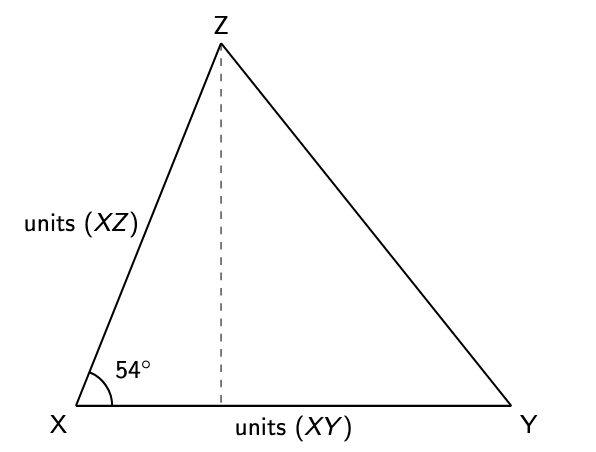
\includegraphics[width=0.45\linewidth]{f9.png}
\end{center}
In triangle $XYZ$, $\angle X = 54^\circ$, $XY = 26$ units, $XZ = 19$ units.

What is the area, in square units, of triangle $XYZ$?

\begin{enumerate}
    \item[A.] 247
    \item[B.] 494
    \item[C.] $247 \sin 54^\circ$
    \item[D.] $494 \sin 54^\circ$
\end{enumerate}
\end{frame}

\begin{frame}{Solution: Triangle Area with Included Angle}
\small
Use the formula:
\[
\text{Area} = \frac{1}{2} ab \sin C
\]

Substitute:
\[
\frac{1}{2} \cdot 26 \cdot 19 \cdot \sin 54^\circ = 247 \sin 54^\circ
\]

\textbf{Answer:} \boxed{\text{C}}
\end{frame}


\newpage
\begin{frame}{\textbf{Question : Circle Geometry and Tangents}}
A circle with center \(O\) has radius \(10\). Point \(A\) lies on the circle, and chord \(AB\) subtends an angle of \(120^\circ\) at the center. A point \(P\) lies on the arc \(AB\), and \(PA\) is extended to meet the tangent to the circle at \(B\) at point \(T\). If \(BT = x\), find the exact value of \(x\).

(\textbf{this question possesses some problems, so just skip that question}
\begin{itemize}
    \item A. \(10\sqrt{3}\)
    \item B. \(15\)
    \item C. \(10\)
    \item D. \(20\)
\end{itemize}
\end{frame}


\begin{frame}{\textbf{Answer to Question }}
We are given:
\[
\angle AOB = 120^\circ, \quad r = 10.
\]
Using the chord length formula:
\[
AB = 2r \sin \left(\frac{\angle AOB}{2}\right) = 2 \cdot 10 \cdot \sin(60^\circ) = 20 \cdot \frac{\sqrt{3}}{2} = 10\sqrt{3}.
\]
Now, applying geometry, since the triangle formed by the radius and the tangent is a right triangle:
\[
OT = 20 \quad \text{(since } OT \text{ is the extension of radius } OP \text{ to the tangent)}
\]
\[
BT^2 = OT^2 - OB^2 = 20^2 - 10^2 = 400 - 100 = 300.
\]
\[
BT = \sqrt{300} = 10\sqrt{3}.
\]

\textbf{Correct Answer: A. \(10\sqrt{3}\)}
\end{frame}





\begin{frame}{\textbf{Question : Triangle in a Semicircle}}
In the figure, \(\triangle ABC\) is inscribed in a semicircle with diameter \(AC = 10\). Point \(B\) lies on the semicircle. If \(AB = 6\) and \(BC = x\), find \(x\). Give your answer in simplest radical form.

\begin{itemize}
    \item A. \(\sqrt{36}\)
    \item B. \(8\)
    \item C. \(\sqrt{44}\)
    \item D. \(\sqrt{64}\)
\end{itemize}
\end{frame}


\begin{frame}{\textbf{Answer to Question }}
By Thales' theorem, any triangle inscribed in a semicircle is a right triangle with the right angle at \(B\). Thus, apply the Pythagorean theorem:
\[
AB^2 + BC^2 = AC^2.
\]
\[
6^2 + x^2 = 10^2 \quad \Rightarrow \quad 36 + x^2 = 100.
\]
\[
x^2 = 64 \quad \Rightarrow \quad x = 8.
\]

\textbf{Correct Answer: B. \(8\)}
\end{frame}



\begin{frame}{\textbf{Question : Intersection of a Parabola and a Circle}}
A parabola is given by 
\[
y = x^2 - 4x + 5,
\]
and a circle by 
\[
x^2 + y^2 = 25.
\]
The parabola and circle intersect at points \(P\) and \(Q\). Find the distance between \(P\) and \(Q\).
(have P)


\end{frame}


\begin{frame}{\textbf{Answer Explanation}}
\textbf{Solution Outline:}
\begin{itemize}
    \item Substitute the expression for \(y\) from the parabola into the circle’s equation:
    \[
    x^2 + (x^2 - 4x + 5)^2 = 25.
    \]
    \item Solve for \(x\) to find the \(x\)-coordinates of the intersection points \(P\) and \(Q\).
    \item Substitute these \(x\)-values back into \(y = x^2 - 4x + 5\) to obtain the corresponding \(y\)-coordinates.
    \item Use the distance formula between \(P(x_1, y_1)\) and \(Q(x_2, y_2)\):
    \[
    \text{Distance} = \sqrt{(x_2 - x_1)^2 + (y_2 - y_1)^2}.
    \]
\end{itemize}

After solving (details omitted for brevity), the distance is found to be:
\[
3.88
\]

\bigskip
\textbf{Correct Answer: 3.88}
\end{frame}

\newpage
\begin{frame}{\textbf{Question  (Be Careful!)}}
Solve the equation:
\[
\sqrt{6r} = \sqrt{r^2 - 16}
\]
What is the product of all solutions to the above equation?
\end{frame}


\begin{frame}{\textbf{Answer to Question }}

\small
\textbf{Step 1:} Square both sides:
\[
6r = r^2 - 16
\Rightarrow r^2 - 6r - 16 = 0
\]

\textbf{Step 2:} Solve the quadratic:
\[
r = \frac{6 \pm \sqrt{(-6)^2 + 4 \cdot 16}}{2}
= \frac{6 \pm \sqrt{36 + 64}}{2}
= \frac{6 \pm \sqrt{100}}{2}
= \frac{6 \pm 10}{2}
\]

\[
\Rightarrow r = 8 \quad \text{or} \quad r = -2
\]

\textbf{Step 3:} Check for extraneous solutions:

Plug into original:
\[
\sqrt{6r} = \sqrt{r^2 - 16}
\]

For \(r = 8\): 
\[
\sqrt{48} = \sqrt{64 - 16} \Rightarrow \sqrt{48} = \sqrt{48} \quad \text{Valid}
\]

For \(r = -2\):
\[
\sqrt{-12} = \sqrt{4 - 16} \Rightarrow \text{Not real} \quad \text{(Invalid)}
\]

\textbf{Only valid solution: } \(r = 8\)

\bigskip
\textbf{Product of all valid solutions: } \( \boxed{8} \)
\end{frame}

\end{document}
